%---------------------------------------------------------------
\chapter{Introduction}
%---------------------------------------------------------------

%--------------------------------
\section{Objectives of the thesis}
%--------------------------------

%The research part of the thesis will describe what is a \gls{puf} and what are the uses of this technology, focusing mainly on \gls{sram} based \glspl{puf}. Furthermore, the parameters used to evaluate performance of \glspl{puf} will be defined.

%The main objective of the practical part of this thesis is to analyze the possibility of implementing a \gls{sram} based \gls{puf} on the ESP32 family of microcontrollers. This means finding a suitable mechanism of \gls{sram} power control and establishing a way to gather \gls{puf} response data reliably. Next, stability and uniqueness of the obtained \gls{puf} data using the defined parameters will be evaluated. An analysis of the \gls{sram} data depending on different operating temperature and power-off time will be performed as well.

%The next goal will be to implement a simple \gls{sram} based \gls{puf} based on the knowledge gained in the previous experiments. Several different models of devices from the ESP32 family will be used to test the function and performance of the resulting \gls{puf} implementation.

\section{Structure of the thesis}

%---------------------------------------------------------------
\chapter{Physical unclonable functions}
%---------------------------------------------------------------

%--------------------------------
\section{PUF description}
%--------------------------------

As \glspl{puf} are the main subject of this thesis, it is important to provide a thorough explanation of what a \gls{puf} is, what types and classes exist and what are
the applications of this technology.

Since more and more types of \glspl{puf} are being invented, it turns out that creating a generalizable description is not a straightforward task. A dictionary definition of a \gls{puf} could be expressed as: \say{a PUF is an expression of an inherent and unclonable instance-specific feature of a physical object}. One can imagine a \gls{puf} being an object's fingerprint in a comparable way to how humans have their own fingerprints.\cite{Maes2013}

The first concept of \gls{puf} was proposed by Pappu in 2001. He used the term \gls{powf}, which he described as a function operating on a physical system that could be easily computed but not easily inverted.\cite{Pappu2001} The first mention of the term \gls{puf} was by Gassend et al.\ in 2002. He talks about \glspl{prf} and a \gls{puf} implementation using \glspl{fpga}.\cite{Gassend2002}

As \gls{puf} is a function, it has inputs and outputs. However, it is not a function in a true mathematical way. It could be described as a procedure performed on a particular device. Its inputs consist of a challenge and a physical state of the device. Given the input, the \gls{puf} produces an output (called a response). Together, they form challenge-response pairs.   

A hugely important property of \glspl{puf} is unclonability. It is achieved by the physical state of the device which acts as the input to the function and influences the responses produced by the \gls{puf}. The concrete details of the physical state used is what distinguishes different \gls{puf} implementations. These physical properties could be for example propagation delay in the chip circuit or bias of uninitialized memory cells to 1 or 0 state. The latter is a basis for \gls{sram} \gls{puf}, which is a topic of this thesis. These properties are fundamentally random since they are created by uncontrollable physical processes during manufacturing. This makes them physically unclonable.

Since the physical state of the device can change with time and environment (for example temperature or input voltage variations), the challenge-response pairs can change as well. The requirement is, that for the same challenge, the responses should be similar enough for us to be able to recognize that they belong to the same challenge. The \gls{puf} responses are also required to differ from device to device even with the same challenge.\cite{Kodytek2020}

Because of these properties, \glspl{puf} can be used in devices to enable secure identification, authentication as well as cryptographic key generation. More of the required properties of \glspl{puf}, their classification, possible applications and implementations will be discussed in more detail in the next sections.

%--------------------------------
\section{PUF properties}
%--------------------------------

In this section, a list of \gls{puf} properties according to~\cite{Maes2012} is described. Some of them are fundamental to all \gls{puf} constructions (the first six listed). However, not all \glspl{puf} must necessarily exhibit all of the discussed properties. In Section~\ref{sec:srampuf_properties}, properties of \gls{sram} \glspl{puf} are discussed as they are a topic of this thesis.

\subsection*{Constructibility}

Constructibility states, that the specific \gls{puf} instance must be `easy' to construct. This means that the laws of physics enable such \gls{puf} implementation in the first place. The construction cost of such \gls{puf} needs to also be adequate for its application.

\subsection*{Evaluability}

The evaluability property discusses the challenge-response mechanism of \glspl{puf}. For a specific challenge, it should be `easy' to obtain the corresponding response. Practically this requires that the response is acquired with respect to time, space, cost and power budget of the application.

\subsection*{Reproducibility}

Reproducibility requires that for a specific \gls{puf} instance, responses produced by the same challenge must be similar enough. The metric that measures the similarity of the responses used is the intra-Hamming distance (which will be defined later in Section~\ref{sec:reliability}). Practically it must be possible to recognize that the responses belong to the same challenge.

\begin{figure}[h!]
    \centering
    \captionsetup{justification=centering,margin=0.5cm}
    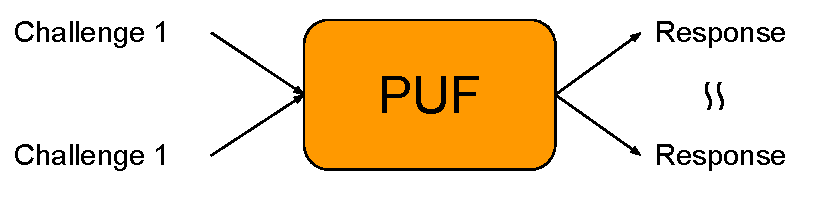
\includegraphics[width=0.75\textwidth]{images/reproducibility}
    \caption{reproducibility: responses to the same PUF challenge need to be similar}
    \label{fig:reproducibility}
\end{figure}

\subsection*{Uniqueness}

While reproducibility talks about the behaviour of a specific \gls{puf}, uniqueness is defined with respect to a set of different \gls{puf} instances. Given the same challenge, two \glspl{puf} must produce a response that is different enough in the given metric. The metric used is the inter-Hamming distance (which will be defined later in Section~\ref{sec:uniqueness}).

\begin{figure}[ht!]
    \centering
    \captionsetup{justification=centering,margin=0.5cm}
    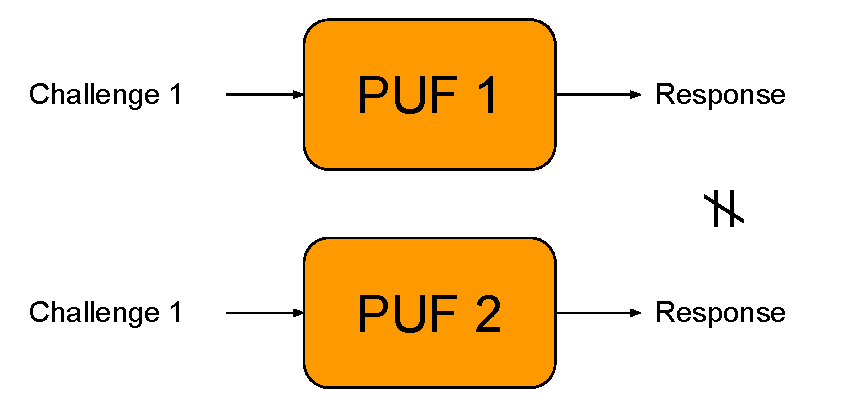
\includegraphics[width=0.75\textwidth]{images/uniqueness}
    \caption{uniqueness: two PUF instances must produce different responses if given the same challenge}
    \label{fig:uniqueness}
\end{figure}

\subsection*{Identifiability}

Identifiability is tied to both uniqueness and reproducibility. Given a single challenge, if the responses from the same \gls{puf} are similar and responses from different \glspl{puf} are different enough, the responses can be used as a means of identification of each \gls{puf}. More formal characterization of the words `similar' and `different' as well as a concrete protocol for \gls{puf} identification is explained in Sections~\ref{sec:puf_evaluation} and~\ref{sec:identification}.

\subsection*{Physical unclonability}
 
Physical unclonability enforces that it is hard to break the uniqueness property. The `hardness' is expressed as a technical and physical infeasibility of creating two nearly identical \gls{puf} instances. In practice, even the manufacturer is unable to break uniqueness due to the uncontrollable physical laws on which the \gls{puf} implementation relies.

\subsection*{Unpredictability}

A \gls{puf} is said to be unpredictable, if given a limited set of challenge-response pairs, it is impossible to create an algorithm that predicts the remaining responses based on a challenge. This means that the challenge-response pair space is sufficiently random.

\subsection*{Mathematical unclonability}

While physical unclonability talks about the impossibility of creating a real-world clone of a specific \gls{puf}, mathematical unclonability requires that no algorithm can predict the \gls{puf} behaviour.

Mathematical unclonability is a stronger model of unpredictability. It assumes unlimited physical access to a specific \gls{puf} instance. The potential adversary can learn as many challenge-response pairs as he is capable of storing and can potentially make use of other \gls{puf} observations. Even in this situation, it should be impossible for the adversary to create a prediction algorithm capable of outputting a response based on a given challenge. 

Mathematical unclonability implies that the specific \gls{puf} implementation has a large number of possible challenges (more than the adversary could theoretically store). If this was not true, a simple lookup table of challenge-response pairs could be constructed, breaking mathematical unclonability. % TODO mention strong PUFs?

\subsection*{True unclonability}

\gls{puf} is considered truly unclonable if it is physically and mathematically unclonable. True unclonability thus implies mathematical and physical unclonability.

\subsection*{One-Wayness}

The one-wayness property is similar to the requirement of cryptographic one-way functions (for example hash functions). Given a \gls{puf} instance and a response, it should be impossible to create an inversion algorithm that can find a corresponding challenge to the response.

Similar to mathematical unclonability, the \gls{puf} needs to have a sufficiently large set of possible challenges and resulting responses in order to meet this property. Otherwise, it would be possible to construct a complete lookup table and find the wanted challenge.

\begin{figure}[h!]
    \centering
    \captionsetup{justification=centering,margin=0.5cm}
    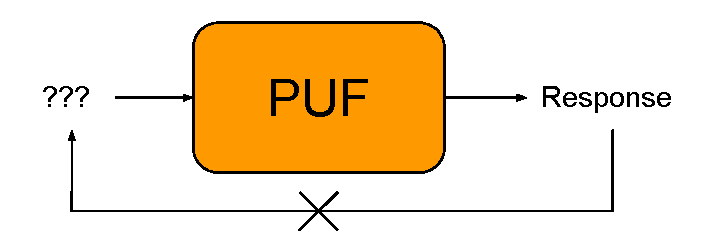
\includegraphics[width=0.75\textwidth]{images/one-wayness}
    \caption{one-wayness: it is impossible to find a challenge corresponding to a given response}
    \label{fig:one-wayness}
\end{figure}

\subsection*{Tamper Evidence}

Tampering with devices in order to compromise their integrity has proven to be a successful technique. For example, invasive attacks (such as microprobing) are able to extract sensitive data from the target system.\cite{Kommerling1999}

Tamper evidence helps to mitigate such attack vectors. The \gls{puf} must detect the attempt to tamper with the system and change its challenge-response pairs to a different set as if the \gls{puf} instance transforms itself to a completely different one.

To achieve this property, the \gls{puf} implementation needs to rely on physical properties that will necessarily change if the device is tampered with. This change will inherently transform the \gls{puf}.

%--------------------------------
\section{PUF classification}
%--------------------------------

A lot of different \gls{puf} implementations have been proposed. They can be classified based on fabrication, security and intrinsic evaluation\cite{Shital2017}\cite{McGrath2019}. A diagram of the discussed \gls{puf} classes is depicted in figure~\ref{fig:classification}.

\begin{figure}[ht!]
    \centering
    \captionsetup{justification=centering,margin=0.5cm}
    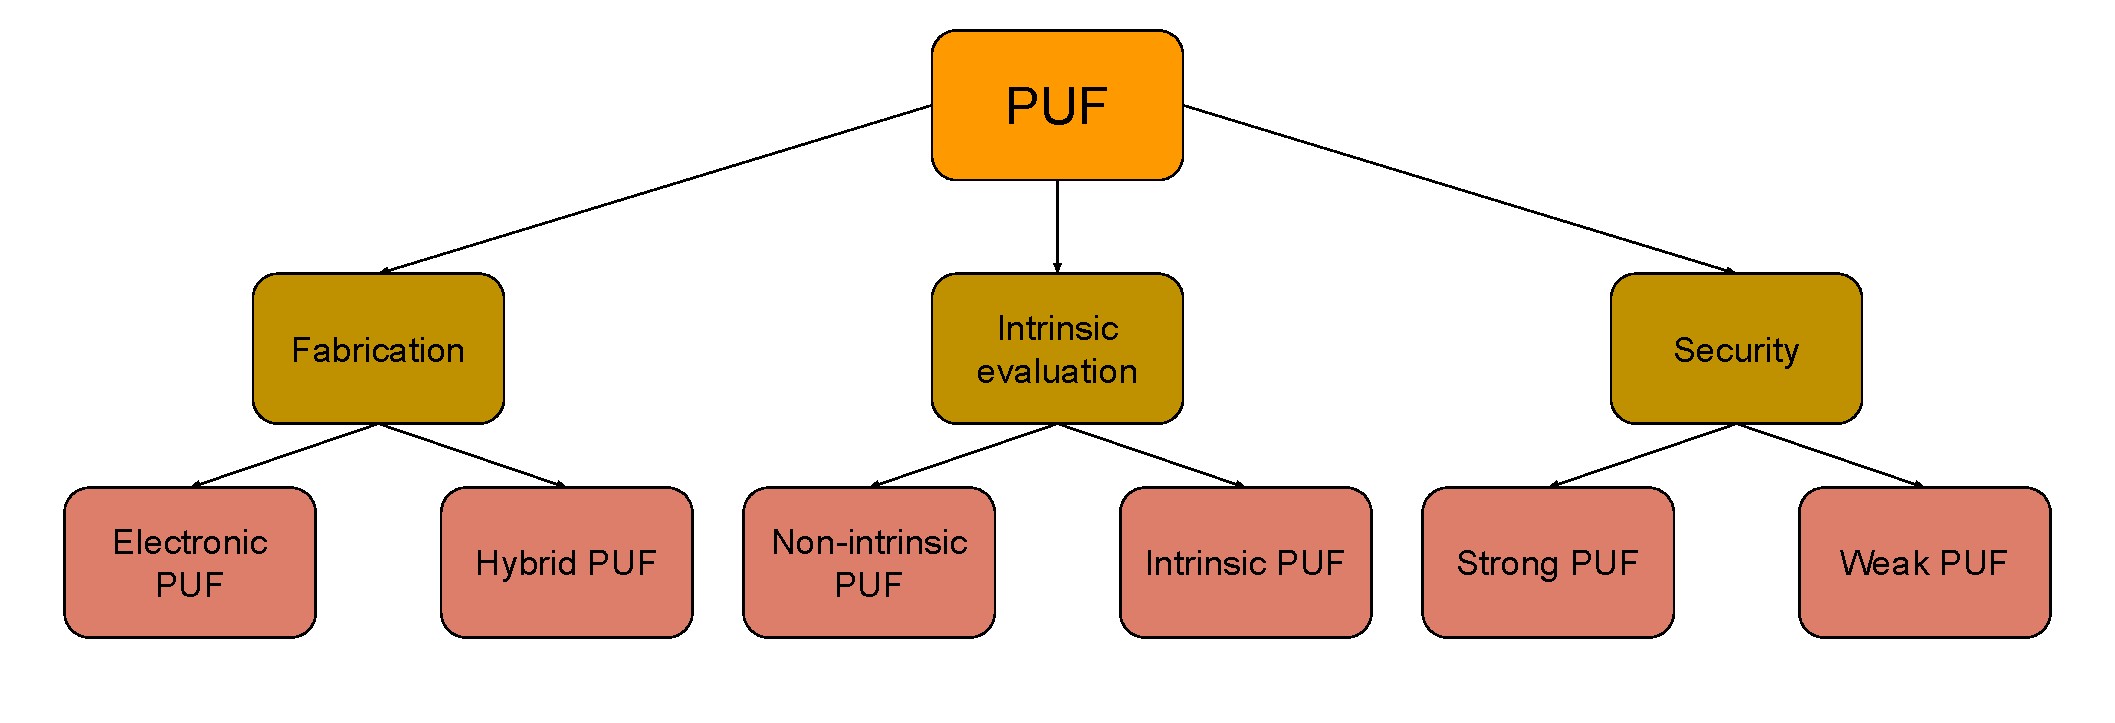
\includegraphics[width=\textwidth]{images/classification}
    \caption{classification of PUFs}
    \label{fig:classification}
\end{figure}

\subsection*{Electronic, silicon and hybrid PUFs}

Electronic \glspl{puf} source their randomness from electronic components. This means that they rely on properties such as capacitance, resistance or propagation delay of a circuit.

A large subclass of electronic \glspl{puf} is silicon \glspl{puf}. They can be constructed only using \gls{cmos} technology, therefore they can be implemented on the same die together with the main chip. This prevents the need to interface with additional circuitry using external buses, lowering cost and limiting the possibility of leaking sensitive data.\cite{Maes2013}

Examples of electronic \glspl{puf} are \gls{sram} \gls{puf}, \gls{ropuf} or arbiter \gls{puf}.

Hybrid \glspl{puf} use non-electronic phenomena to create their challenge-response pairs. While randomness introduced into the system is of non-electronic nature, the signal is usually processed and stored using electronic components. Hence the name hybrid \glspl{puf}. They can be based on optics (optical \gls{puf}), magnetism (magnetic \gls{puf}) or quantum effects (quantum \gls{puf}\cite{Koustubh2021}).


\subsection*{Intrinsic and non-intrinsic PUFs}

A \gls{puf} implementation is said to be intrinsic if it satisfies the following two conditions:

\begin{enumerate}
    \item responses are evaluated internally
    \item instance-specific random features are introduced implicitly during the manufacturing process
\end{enumerate}

Internal evaluation requires the measurement equipment of the \gls{puf} to be embedded in the device. This, similar to silicon \glspl{puf}, lowers cost and is more secure.

The second condition discusses the introduction of randomness into the system. Implicit randomness relies on process variations taking place during normal manufacturing, while explicit randomness needs to be created by special procedures which would have not been needed otherwise (such as doping with random dielectric particles for the construction of a coating \gls{puf}\cite{Kori2006}).

\gls{sram} and arbiter \glspl{puf} are examples of intrinsic \glspl{puf}. If the \gls{puf} construction does not satisfy the given properties, it is called non-intrinsic. For example, optical or coating \glspl{puf} are non-intrinsic.\cite{Maes2012}

\subsection*{Strong and weak PUFs}

Security based classification distinguishes \gls{puf} implementations according to the size of their challenge-response pair sets.

In order for a \gls{puf} to be classified as strong, its challenge-response pair set needs to be sufficiently large to prevent an exhaustive search by a possible attacker. The challenge-response pair size thus scales well (preferably exponentially) with some construction parameter.\cite{Guajardo2007}

On the other hand, weak \glspl{puf} have only a limited set of challenge-response pairs. Some \glspl{puf} can only have one pair. They are sometimes called \gls{pok}.

As the naming implies, strong \gls{puf} constructions possess, in some sense, greater security. Weak \glspl{puf} cannot be mathematically unclonable (and consequently cannot be truly unclonable or unpredictable). Strong \glspl{puf} can also be used in more applications, as explained in Section~\ref{sec:puf_applications}. However, it turns out that constructing a strong \gls{puf} is a very hard problem.\cite{Maes2013}

%--------------------------------
\section{PUF evaluation parameters}\label{sec:puf_evaluation}
%--------------------------------

\subsection{Uniformity}
\subsection{Uniqueness}\label{sec:uniqueness}
\subsection{Reliability}\label{sec:reliability}
\subsection{?Randomness}

%--------------------------------
\section{PUF applications}\label{sec:puf_applications}
%--------------------------------

\subsection{Identification}\label{sec:identification}
\subsection{Authentication}
\subsection{Key generation}

%--------------------------------
\section{PUF implementations}
%--------------------------------

\subsection{Optical PUF}\label{sec:optical_puf}
\subsection{SRAM PUF}
\subsubsection*{SRAM PUF and its properties}\label{sec:srampuf_properties}

%---------------------------------------------------------------
\chapter{ESP32 platform}
%---------------------------------------------------------------

%---------------------------------------------------------------
\chapter{SRAM PUF implementation on ESP32}
%---------------------------------------------------------------

%--------------------------------
\section{RTC SRAM based PUF}
%--------------------------------

\subsection{RTC SRAM power control}
\subsection{SRAM analysis based on temperature and power off time}
\subsection{PUF evaluation parameters}

%--------------------------------
\section{Deep sleep based PUF}
%--------------------------------

\subsection{Deep sleep SRAM power control}
\subsection{SRAM analysis based on temperature and power off time}
\subsection{PUF evaluation parameters}

%--------------------------------
\section{?PUF response data image} % TODO how to name this section?
%--------------------------------

%---------------------------------------------------------------
\chapter{Reliable PUF response extraction} % TODO should this be its own section or part of the previous one?
%---------------------------------------------------------------

%--------------------------------
\section{Stable bits selection}
%--------------------------------

%--------------------------------
\section{Error correction code}
%--------------------------------

%--------------------------------
\section{Provisioning}
%--------------------------------

%--------------------------------
\section{Combining power control methods}
%--------------------------------

%--------------------------------
\section{Reliability testing}
%--------------------------------

%---------------------------------------------------------------
\chapter{ESP32 SRAM PUF library}
%---------------------------------------------------------------

%---------------------------------------------------------------
\chapter{Conclusion}
%---------------------------------------------------------------

